\documentclass[aps,pra,twocolumn,superscriptaddress,longbibliography,floatfix,nofootinbib]{revtex4-2}

\usepackage{amsmath,amssymb,amsfonts}
\usepackage{graphicx}
\usepackage[dvipsnames]{xcolor}
\usepackage{hyperref}
\usepackage{booktabs}
\usepackage{bm}
\usepackage{mathtools}

\providecommand{\ket}[1]{\lvert #1 \rangle}
\providecommand{\bra}[1]{\langle #1 \rvert}

\hypersetup{
  colorlinks=true,
  linkcolor=blue!60!black,
  citecolor=blue!60!black,
  urlcolor=blue!60!black,
  pdfauthor={Berkay Y{\"u}ksel Sayim},
  pdftitle={Correlation Witnesses versus Magic: A k-Resolved Nonstabilizerness Map for SU(2)_k Anyon Fusion Spaces},
  pdfsubject={quant-ph},
  pdfkeywords={nonstabilizerness, magic, Bell inequality, Leggett-Garg
               inequality, KCBS, anyons, SU(2)_k, topological quantum
               computation, stabilizer Renyi entropy}
}

\begin{document}

\setcounter{secnumdepth}{3}

\title{Correlation Witnesses versus Magic: A $k$-Resolved Nonstabilizerness Map for $\mathrm{SU}(2)_k$ Anyon Fusion Spaces}

\author{Berkay Y\"uksel Sayim}
\email{berksa@tutamail.com}
\affiliation{Independent Research, Germany}
\affiliation{\href{https://orcid.org/0009-0004-4993-7352}{ORCID:
0009-0004-4993-7352}}

\date{2026-09-22}

\begin{abstract}
Standard correlation witnesses --- spatial Bell/CHSH inequalities,
temporal Leggett--Garg $K_3$, and KCBS contextuality --- are known to
detect nonstabilizerness (``magic'') in some settings. We report a
worked example, a $k$-resolved nonstabilizerness map of the
$\mathrm{SU}(2)_k$ anyon braid-representation family, in which a
standard temporal witness is instead systematically \emph{blind}: at
$k=4$ the three-time Leggett--Garg witness saturates its
macrorealistic bound exactly ($K_3=1.000000$ over every state, braid
element, and measurement axis) in the equal-time-step protocol of
Table~\ref{tab:map} ($V_1{=}V_2$), while the single-qubit fusion channel
carries near-maximal nonstabilizerness ($M_2=0.5585$, $95\%$ of the
finite-dimensional ceiling $\log_2(3/2)$). We prove this blindness as
a structural theorem: the witness depends only on the Bloch-sphere
Gram geometry of the braid orbit, not on nonstabilizerness, and $k=4$
happens to align the fixed measurement axis with a threefold orbit
symmetry (Bloch dot products all $-1/3$) that caps the witness at
$1$; a finite, Clifford-generating group --- the chiral octahedral
group, the $k{=}2$ braid image --- with a misaligned axis reaches
$K_3=3/2$ under a two-propagator protocol. Neither finiteness of the braid image nor the
Clifford property is by itself the mechanism. We complement this
temporal certificate with three independent certificates of genuine
nonstabilizerness --- two of them long-range (a doubled-Fibonacci
mutual-information witness, $H=1.700979$, and a gauge-invariant minimum
ground-space stabilizer Rényi entropy, $\geq6.5$ against an exact-zero
toric-code control), the third a complementary gate-based
non-Cliffordness measure --- an honest negative
control confirming that leakage-free constructions remain strictly
additive, and a hardware-oriented single-qubit signal-to-noise
prediction. We further pair the $k=4$ dissociation with Kochen--Specker--Klyachko
contextuality at their shared $d=3$ interface, where the KCBS witness certifies
contextuality yet shows only a weak, nongeneric correlation with magic. Two reconciliations with the literature are made explicit: the present result contradicts
neither the equivalence of maximal nonlocality and maximal magic established for optimized magic
states in a different game, nor the contextuality-supplies-magic theorem; both concern a
different object than the fixed, per-$k$ braid generator studied here.
\end{abstract}

\keywords{nonstabilizerness; magic; Bell inequality; Leggett-Garg
inequality; KCBS; anyons; SU(2)$_k$; stabilizer Renyi entropy}

\maketitle

%% ====================================================================
\section{Introduction and related work}
\label{sec:intro}

Nonstabilizerness, or ``magic,'' is the resource that lifts Clifford
circuits to universal quantum computation~\cite{VeitchEtAl2014,%
HowardCampbell2017}, and it is by now well established that standard
Bell-type correlation witnesses can \emph{detect} it: Macedo \emph{et
al.}~\cite{Macedo2025} and Cusumano \emph{et
al.}~\cite{Cusumano2026} both construct Bell inequalities whose
violation certifies nonstabilizerness, and the Ising-anyon no-go of
Howard and Vala~\cite{HowardVala2012} shows, in the opposite direction,
that Clifford-only (Ising) braiding transformations cannot violate a
Bell inequality when only topologically protected stabilizer operations
are performed. Both directions concern whether, and how, a
correlation witness sees magic. A companion paper realizes exactly
the Howard--Vala Ising setting microscopically, on a concrete Kitaev
honeycomb Hamiltonian, showing that the noncommuting CHSH
Bell-operator \emph{algebra} is realized locally while a genuine
physical violation is not~\cite{Sayim2026witness}; the magic resource
whose presence or absence that companion paper's argument turns on is
exactly the subject of the present paper, and we cross-reference it
bidirectionally throughout.

This paper reports the complementary direction, a \emph{blind spot}:
a standard correlation witness --- the temporal Leggett--Garg
inequality $K_3\le1$~\cite{LeggettGarg1985,Budroni2014} --- fails to
detect near-maximal single-qubit magic present in a specific,
structurally identified member of the $\mathrm{SU}(2)_k$
braid-representation family, at $k=4$. This is not a new claim that
correlation witnesses can be blind to magic \emph{in general} ---
Howard and Vala already establish an instance of witness blindness for
Ising braiding~\cite{HowardVala2012} --- but a $k$-resolved,
numerically exhibited, and structurally explained dissociation map
across the $\mathrm{SU}(2)_k$ family, together with three independent
certificates of genuine nonstabilizerness (two long-range, the third
a complementary gate-based measure) and an honest negative
control. We stress at the outset what this paper is \emph{not}: it is
not a claim that magic is generically decoupled from Bell/CHSH
correlations --- Macedo and Cusumano show the opposite in their
respective constructions --- and the present $k=4$ result is the
complementary blind spot on a single, finite braid generator, not a
general no-go. A related but distinct construction, Robin and
Savage's anti-flatness witness of nonlocal magic in two-particle
scattering~\cite{RobinSavage2025}, cites the same spatial
magic--CHSH suppression as Macedo and Cusumano but treats a
different Hilbert space (a two-qubit scattering channel, not anyons
or an $\mathrm{SU}(2)_k$ family) and does not touch the temporal or
$k$-resolved question studied here; we note it as related work
rather than a competing claim.

An independent line of work develops a general recipe for turning
standard tomographic measurements into tailored Bell inequalities and
applies it to witness magic: Cie\'sli\'nski \emph{et
al.}~\cite{Cieslinski2026} show that the same Pauli-basis measurements
routinely taken for state tomography certify nonlocality at no
additional experimental cost, and, noting the stabilizer structure of
the resulting inequalities, use them as magic witnesses. This is again a
\emph{detection} result for a spatial (Bell-type) witness, on a
general multi-qubit tomographic setting rather than an anyon
braid-representation platform; it does not address the temporal
Leggett--Garg witness or the $k$-resolved dissociation that is the
subject of the present paper.

Two further reconciliations, closer to the present claim than the
detect/blind distinction above, are necessary before we can state the
$k=4$ result without ambiguity. Howard~\cite{Howard2015} proves an
\emph{equivalence} between maximum nonlocality and maximum magic in a
qudit CHSH-type game optimized over the magic \emph{state}: this
sounds directly opposed to any witness/magic dissociation. The
distinction is the object being varied. Howard's equivalence concerns
the optimal single-qudit magic \emph{state} in a fixed correlation
game; the present $k=4$ result concerns a fixed \emph{braid generator}
(no state optimization) at one specific value of the family index $k$,
evaluated as a witness of whichever magic that braid generator's
fusion channel happens to carry. The two are different optimization
problems over different objects, and neither result constrains the
other. Second, Howard, Wallman, Veitch, and
Emerson~\cite{HWVE2014} prove that contextuality is necessary for the
magic-state resource that promotes stabilizer computation to
universality (odd-prime local dimension). We report below
(Sec.~\ref{sec:t5}) a near-zero, nongeneric correlation between a
KCBS contextuality witness and magic at $k=4$; this is not in tension
with the HWVE theorem. HWVE is a global existence/threshold statement
about universality (odd-prime local dimension), whereas our KCBS
correlation is a pointwise measurement over one finite-$k$ orbit, not
a threshold claim. The separate blindness of our temporal $K_3$
witness (Secs.~\ref{sec:map}--\ref{sec:theorem}) is of a different
character still: $K_3$ is a temporal witness, not a spatial/polytope
contextuality inequality, and the $k=4$ dissociation is a structural
corollary of a single braid generator being a $z$-axis rotation, not
a general statement about contextuality and magic.

The rest of this paper is organized as follows. Section~\ref{sec:axes}
fixes five nonstabilizerness axes and the $\log_2$ convention used
throughout. Section~\ref{sec:map} presents the $k$-resolved
dissociation map, Fig.~\ref{fig:map}, with the $k=4$ blind spot as the
central result. Section~\ref{sec:theorem} proves the blindness as a
structural theorem. Section~\ref{sec:lrn} reports three independent
certificates of nonstabilizerness --- two long-range and a
complementary gate-based axis. Section~\ref{sec:n1} reports
an honest negative control. Section~\ref{sec:hw} gives a
single-qubit hardware signal-to-noise prediction.
Section~\ref{sec:t5} maps the dissociation onto an interface with
KCBS contextuality, left open here,
and states the scope limitations of this work.

%% ====================================================================
\section{Five nonstabilizerness axes}
\label{sec:axes}

We fix one convention throughout: all magic monotones are reported in
base-2 logarithm (bits), following the resource-theoretic construction
of Veitch \emph{et al.}~\cite{VeitchEtAl2014},
$M(\rho)=\log_2\bigl(1+2\,\mathrm{sn}(\rho)\bigr)$, where
$\mathrm{sn}(\rho)$ is the sum-negativity of the discrete Wigner
representation of $\rho$. Byles, Forbes, and
Pachos~\cite{Byles2024} report the qutrit gate-magic value
$M_2=\log(16/13)$ without specifying the logarithm base; in base 2
this is $M_2=\log_2(16/13)=0.2996$, the value we cite below. The five
axes evaluated across the $\mathrm{SU}(2)_k$ family are: (1) the
stabilizer $2$-Rényi entropy (SRE) $M_2$~\cite{LeoneOlivieroHamma2022},
proven to be a genuine magic monotone for Rényi index $\alpha\ge2$ by
Leone and Bittel~\cite{LeoneBittel2024}, of the single-qubit
braid-generator fusion channel (state magic); (2) the robustness of
magic (RoM)~\cite{HowardCampbell2017}; (3) the amortized, gate-based
non-Cliffordness of the braid generator itself (Sec.~\ref{sec:map});
(4) the two independent long-range-nonstabilizerness certificates of
Sec.~\ref{sec:lrn} (which additionally re-presents axis~(3) as a
complementary third non-Cliffordness check); and (5) the temporal
Leggett--Garg witness $K_3$
and the KCBS contextuality witness of Sec.~\ref{sec:t5}, both used as
correlation witnesses rather than magic monotones. An independent,
sampling-based route to the same family of monotones is Bell
sampling~\cite{HaugKim2023}, which we do not use directly but note as
an alternative, hardware-compatible estimator.

%% ====================================================================
\section{The $k$-resolved dissociation map}
\label{sec:map}

For each $k$ we consider the standard $\mathrm{SU}(2)_k$ braid
generator acting on a single fusion-channel qubit as a $z$-axis
rotation by the level-dependent angle
$\theta_k=\pi(k+4)/(k+2)$~\cite{FreedmanLarsenWang2002,%
FreedmanLarsenWang2003}; the braid image is dense in
$\mathrm{SU}(2)$ for every $k\ge2$ with $k\notin\{2,4,8\}$~\cite{Kuperberg2011}
(density alone, not finiteness, is the relevant classification for
the ``dense'' rows of Table~\ref{tab:map} below). We evaluate,
independently, a correlation
witness (the temporal Leggett--Garg $K_3$) and three magic monotones
(the stabilizer $2$-Rényi entropy $M_2$, the robustness of magic RoM,
and the amortized gate-based non-Cliffordness of
Sec.~\ref{sec:theorem}) across $k=2,\ldots,10$. Table~\ref{tab:map}
and Fig.~\ref{fig:map} report all four quantities; the three magic
monotones, evaluated by an independent re-implementation cross-checked
by two further computations sharing verified conventions, give a
concordant classification across the family --- each sits at its own
no-magic value at $k=2$, lies strictly above it at every higher level,
and drops at the two levels whose braid image is finite --- although
their numerical ranges differ (for $M_2$: the Clifford floor $0$ at
$k=2$, a finite non-Clifford plateau at $k=4,8$, and the
dense-representation ceiling $\log_2(3/2)=0.585$ approached at
$k=3,5,6,7,9,10$), and the two $K_3$ columns
(state- and axis-optimized $K_3^{\mathrm{opt}}$, versus the
fixed-measurement-axis value $K_3(Q{=}\hat z)$ used operationally in
Sec.~\ref{sec:theorem}) agree everywhere except at $k=8$, where the
two differ by construction (Sec.~\ref{sec:theorem}, scope remark).

\begin{table}[!h]
\centering
\caption{$k$-resolved dissociation map. FLW: dense in
$\mathrm{SU}(2)$ (Freedman--Larsen--Wang universality); for $k\ge2$,
finite braid images occur only at $k\in\{2,4,8\}$~\cite{FreedmanLarsenWang2002},
corresponding to the binary polyhedral groups $2O,2T,2I$ of orders
$48,24,120$ (McKay correspondence with the $E_7,E_6,E_8$ Dynkin
diagrams). $K_3^{\mathrm{opt}}$: Leggett--Garg witness in the
equal-time-step protocol ($V_1{=}V_2$), maximized over states and
measurement axis, and over the full braid image for the finite cases
$k=2,4,8$; for the dense cases by random-word sampling, which
approaches but cannot attain the supremum. $K_3(Q{=}\hat z)$: same
witness at the fixed measurement axis used in Sec.~\ref{sec:theorem}.
$M_2$: stabilizer $2$-Rényi entropy (state magic, $\log_2$). RoM:
robustness of magic. All values reproduced by an independent
re-implementation and cross-checked by two further evaluations sharing
verified conventions; $\lvert\Delta\rvert\le10^{-6}$ throughout.}
\label{tab:map}
\begin{tabular}{cccccc}
\toprule
$k$ & finite image & $K_3^{\mathrm{opt}}$ & $K_3(Q{=}\hat z)$ & $M_2$ & RoM \\
\midrule
2 & $2O$ (48)  & $1.000$ & $1.000$ & $0.000$ & $1.000$ \\
3 & dense      & $1.500$ & $1.498$ & $0.585$ & $1.732$ \\
\textbf{4} & $\bm{2T}$ \textbf{(24)} & \textbf{1.000} & \textbf{1.000} & \textbf{0.5585} & \textbf{1.715} \\
5 & dense      & $1.500$ & $1.479$ & $0.585$ & $1.732$ \\
6 & dense      & $1.500$ & $1.495$ & $0.584$ & $1.732$ \\
7 & dense      & $1.498$ & $1.494$ & $0.585$ & $1.732$ \\
8 & $2I$ (120) & $1.427$ & $1.342$ & $0.5530$ & $1.714$ \\
9 & dense      & $1.500$ & $1.497$ & $0.585$ & $1.732$ \\
10 & dense     & $1.500$ & $1.491$ & $0.585$ & $1.732$ \\
\bottomrule
\end{tabular}
\end{table}

\begin{figure}[!h]
\centering
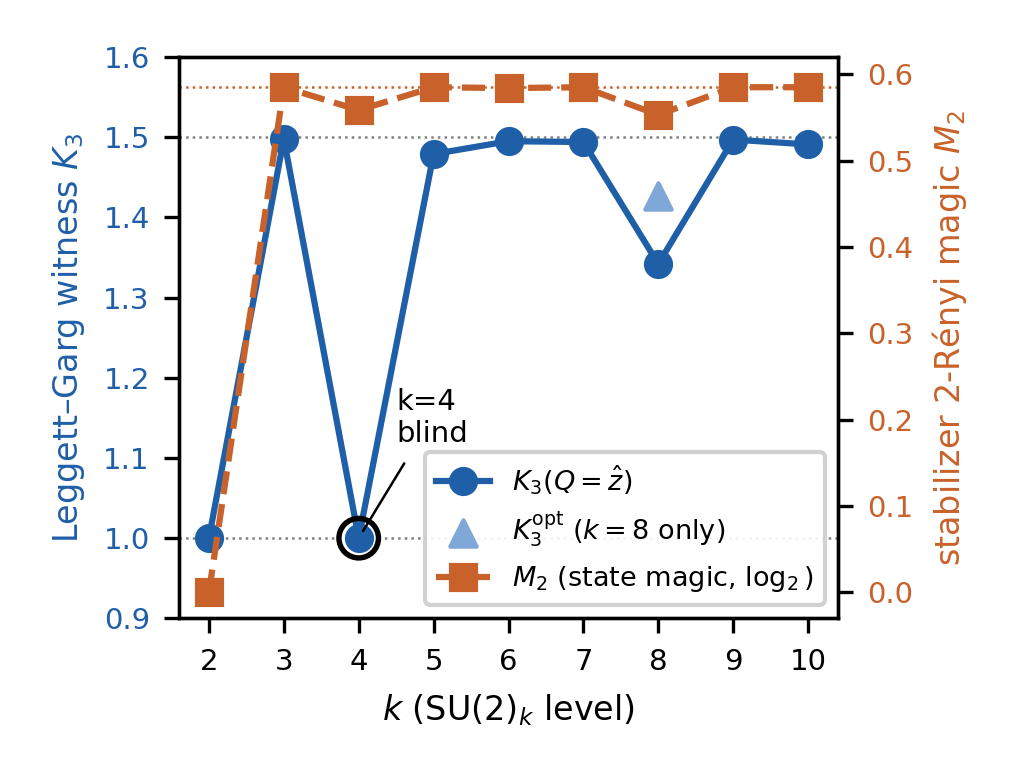
\includegraphics[width=\columnwidth]{p5a_fig1_dissociation_map.png}
\caption{The $k=4$ dissociation. Top: Leggett--Garg witness
$K_3(Q{=}\hat z)$ (blue) against stabilizer $2$-Rényi magic $M_2$
(orange, $\log_2$ basis) across $k=2,\ldots,10$. At $k=4$ the witness
sits at its macrorealistic ceiling, $K_3=1.000$ (open circle, blind),
while $M_2=0.5585$ is at $95\%$ of the dense-representation ceiling
$\log_2(3/2)=0.585$ (dashed line). At $k=2$ the witness is likewise at
its bound, but there is no magic to miss ($M_2=0$); at every dense $k$
and at $k=8$ it exceeds the classical bound. The dissociation is
specific to $k=4$: witness silent, resource present.
The $k=8$ point shows the fixed-axis value $K_3(Q{=}\hat z)$;
the axis-optimized value $K_3^{\mathrm{opt}}=1.427$ (Table~\ref{tab:map})
is shown as a lighter marker for comparison.}
\label{fig:map}
\end{figure}

The central object of this paper is the $k=4$ column of
Table~\ref{tab:map}: the Leggett--Garg witness is pinned at its
macrorealistic bound, $K_3=1.000000$, over \emph{every} state, every
braid word, and every measurement axis in the equal-time-step
protocol ($V_1{=}V_2$). The axis-sweep is a genuine
numerical search, not a fixed-axis artifact --- the same
axis-optimization protocol applied at $k=8$ (Sec.~\ref{sec:theorem})
finds a strictly larger value there, $1.427$ against the fixed-axis
$1.342$, so the search demonstrably explores nonaligned axes and
still finds no $k=4$ violation. The closed-form Gram-geometry argument
of Sec.~\ref{sec:theorem} independently explains \emph{why} the
physical, fixed measurement axis used throughout this paper gives
exactly $1$ at $k=4$ (it is aligned with a threefold orbit symmetry).
In the equal-time-step protocol of Table~\ref{tab:map} ($V_1{=}V_2$)
the $k=4$ blindness holds for \emph{every} measurement axis, a closed
result established for the companion $\mathrm{SU}(2)_k$ Leggett--Garg
witness~\cite{Sayim2026SU2k} (its $M(U)$ eigenvalues exceed $1$ only
for rotation angles in $(0^\circ,90^\circ)$, which the tetrahedral
group does not contain); under the more general two-propagator
protocol of Sec.~\ref{sec:theorem} the blindness is instead bound to
alignment, and a misaligned axis reaches $K_3=3/2$ --- the alignment
mechanism itself, not a defect.

Meanwhile, the maximum state magic accessible over the $k=4$
braid-image orbit reaches $M_2=0.5585$, i.e.\ $95\%$ of the
finite-dimensional ceiling
$\log_2(3/2)=0.585$ approached by the dense representations, and a
robustness of magic $\mathrm{RoM}=1.715$ close to the dense ceiling
$\sqrt3=1.732$. We stress the framing: $K_3=1$ at $k=4$ is a
\emph{single-qubit corollary} of a specific braid rotation angle, not
a new physical phenomenon, and the finding is that the witness misses
a resource that is, by every available magic monotone, almost as
large as it can be for this family.

%% ====================================================================
\section{Structural theorem: alignment, not finiteness or Clifford}
\label{sec:theorem}

We now explain the $k=4$ blind spot as a theorem rather than a
numerical coincidence. Consider the temporal Leggett--Garg protocol
with a fixed dichotomic observable $Q=\hat n_0\!\cdot\!\bm\sigma$
(here $\hat n_0=\hat z$) and two independent propagators $V_1,V_2$
drawn from a group $G\subset\mathrm{SU}(2)$, giving Heisenberg
observables $Q_1=Q$, $Q_2=V_1^\dagger QV_1$, $Q_3=(V_2V_1)^\dagger
Q(V_2V_1)$ with Bloch directions $\hat n_1=\hat n_0,\hat n_2,\hat
n_3$ in the orbit of $\hat n_0$ under the $\mathrm{SO}(3)$ image of
$G$. For any single-qubit dichotomic pair,
$\{\hat n\!\cdot\!\bm\sigma,\hat m\!\cdot\!\bm\sigma\}
=2(\hat n\!\cdot\!\hat m)\openone$, so the Lüders two-time
correlator reduces to a Bloch dot product independent of the state,
\begin{equation}
\label{eq:gram}
C_{ij} = \hat n_i\cdot\hat n_j \qquad \text{for every } \rho,
\end{equation}
and consequently
$K_3^{\max}=\max_{(\hat n_2,\hat n_3)\in\text{orbit}}
(\hat n_1\!\cdot\!\hat n_2+\hat n_2\!\cdot\!\hat n_3-\hat n_1\!\cdot\!\hat n_3)$
depends only on the Gram matrix of Bloch dot products within the
orbit of $\hat n_0$ under $G$ --- \emph{not} on whether the braid
representation is finite, and not on whether $G$ is a Clifford
subgroup. The real $k=4$ braid image is the binary tetrahedral group
$2T$ (projective order $12$), and $\sigma_1$ acts as a projective
threefold rotation about $\hat z$: the orbit of $\hat z$ under the
full projective group $2T$ is exactly the four vertices of a
tetrahedron, with every
off-diagonal Bloch dot product equal to $-1/3$. Exhaustive
enumeration over the $4^2=16$ orbit pairs (with $\hat n_1=\hat n_0$
fixed) gives $K_3^{\max}=1$ exactly, matching Table~\ref{tab:map}. The same
Gram argument applied to the real $k=8$ braid image (binary
icosahedral group $2I$, twelve icosahedral Bloch directions, dots
$\{\pm1,\pm1/\sqrt5\}$) gives $K_3^{\max}=3/\sqrt5=1.341641$ in the
fixed-$\hat z$-axis protocol, and $K_3^{\mathrm{opt}}=2\cos72^\circ
-\cos144^\circ=1.427$ under the axis-optimized protocol in which the
measurement axis is rotated to be perpendicular to a fivefold orbit
axis unreachable from the fixed $\hat z$ frame --- the two $k=8$
numbers in Table~\ref{tab:map} differ by measurement-protocol scope,
not by inconsistency.

The corollary that gives this theorem its bite is a direct
counterexample to the plausible-sounding slogan ``a finite braid image
or a Clifford-generating group is witness-blind'': the chiral
octahedral group ($24$ elements, itself a genuine single-qubit
Clifford subgroup) with the measurement axis \emph{rotated} to
$\hat n_0=(1,1,0)/\sqrt2$ instead of a coordinate axis has orbit dots
$\{0,\pm\tfrac12,\pm1\}$ and reaches $K_3^{\max}=3/2$ exactly, the full
Lüders bound --- realized operationally by two genuine $\mathrm{SU}(2)$
qubit unitaries reproducing the same value to machine precision. The
same finite, Clifford-generating group is witness-blind at one axis
and witness-saturating at another; neither finiteness nor the
Clifford property is the driver. The same conclusion follows across
levels rather than across axes (Fig.~\ref{fig:orbit}): the three
levels with a finite braid image do not share a verdict, their group
orders are not ordered along $k$, and the two levels closest in magic
lie on opposite sides of the bound. What is sufficient for blindness is
\emph{alignment}: the fixed measurement axis coincides with a symmetry
axis of the orbit whose Gram structure caps the witness (here, $\hat z$
is the threefold axis of the $k=4$ tetrahedral orbit, with all Bloch
dot products $-1/3$), forcing the
orbit Gram matrix into a form whose maximum is exactly $1$. We
emphasize, following the explicit abstraction argument, that
Gottesman--Knill classical simulability of Clifford circuits is not
invoked anywhere in this argument and does not by itself imply
Leggett--Garg inertness; the mechanism is the Bloch-sphere Gram
geometry of the orbit, evaluated in Eq.~\eqref{eq:gram}, not
computational-complexity simulability. Correspondingly, the correct
statement of the $k=4$ result is that \emph{this witness measures
orbit alignment, not magic or universality}; it says nothing about
other witnesses or other measurement axes.

\begin{figure}[!h]
\centering
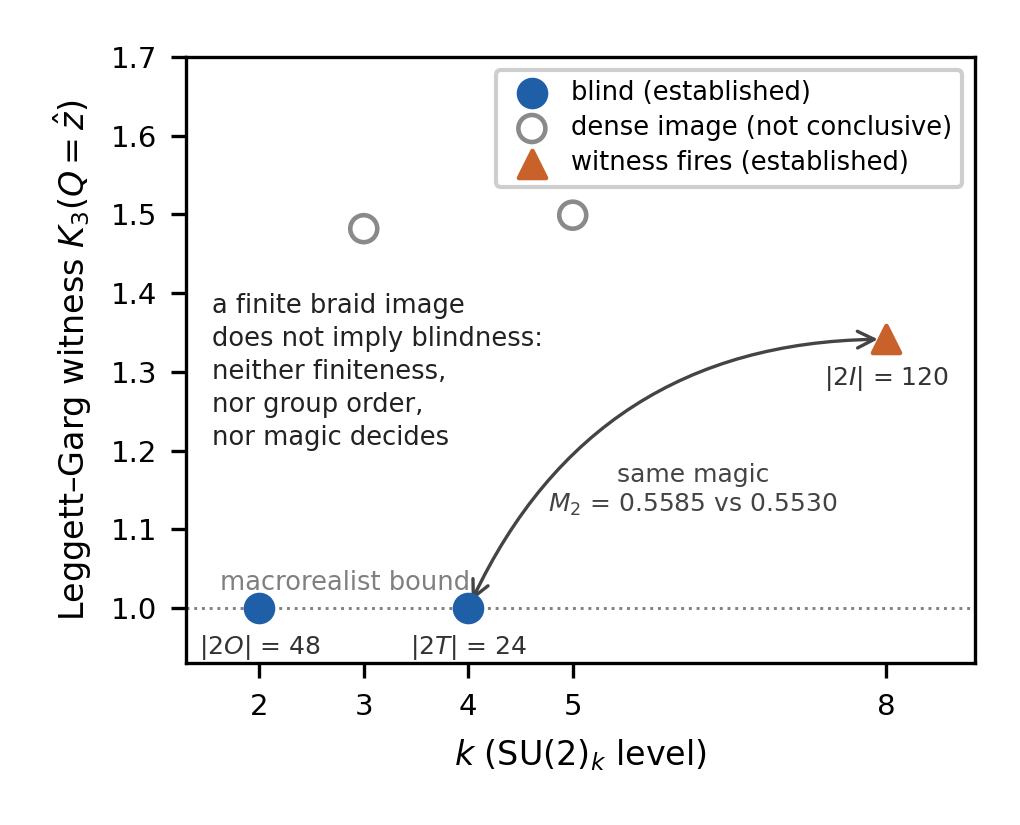
\includegraphics[width=\columnwidth]{p5a_fig2_orbit_geometry.png}
\caption{What does \emph{not} decide blindness. Fixed-axis
Leggett--Garg witness $K_3(Q{=}\hat z)$ against the level $k$, for the
three levels with a finite braid image ($k=2,4,8$; filled markers,
group orders in the binary convention of Table~\ref{tab:map}) together
with two dense levels shown for reference ($k=3,5$; open markers,
sampling-dependent and therefore not conclusive). The orders are not
ordered along $k$ ($48\to24\to120$), and $k=4$ and $k=8$ carry nearly
the same magic ($M_2=0.5585$ against $0.5530$) while lying on opposite
sides of the macrorealistic bound. The dense levels are kept in the
figure because they are the evidence for their own exclusion: among
the three finite levels alone, other columns of the deposited data
would appear to separate the verdicts. What does decide --- alignment
of the fixed axis with an orbit symmetry axis whose Gram structure
caps the witness --- is stated in the text above; no column of the
deposited data carries it as a scalar, so it is not drawn here. All
plotted values are read from \texttt{p5a\_ergebnis\_t4.json}.}
\label{fig:orbit}
\end{figure}

%% ====================================================================
\section{Three certificates of genuine nonstabilizerness}
\label{sec:lrn}

Beyond the single-qubit dissociation of Secs.~\ref{sec:map}--\ref{sec:theorem},
we report three methodologically independent certificates of genuine
nonstabilizerness, in the same spirit as the exact SU(2)$_k$ mana
computation of Fliss~\cite{Fliss2021}, the exact-setting anchor we
follow most closely among prior anyon-magic constructions. The first
two, (1) and (2), certify genuine \emph{long-range} (many-body,
topologically encoded) magic not reducible to a local artifact; the
third, (3), is the complementary gate-based non-Cliffordness axis of
the map (axis~(3), Sec.~\ref{sec:axes}) --- a single-generator
quantity included here as a methodologically distinct third line of
non-Cliffordness evidence, not a long-range-state certificate in the
sense of (1)--(2). Each of the two long-range certificates is a
\emph{sufficient} condition for genuine long-range magic (a
noninteger witness value, or a gauge-invariant lower bound bounded
away from zero); we make no claim that either is \emph{necessary}, and
do not rule out other long-range-magic witnesses that these two
constructions happen to miss.

These certificates are not offered as a priority claim on the presence
of long-range nonstabilizerness in this class --- for the two
long-range certificates (1) and (2) that statement is the theorem of
Zhang \emph{et al.}~\cite{Zhang2026} quoted below --- but as the
quantitative substrate for the dissociation of
Secs.~\ref{sec:map}--\ref{sec:theorem}: they establish, with explicit
values and null controls, the magic that the temporal witness
demonstrably fails to detect. Certificate (3) is not covered by that
theorem at all: it is a gate-based measure, whereas Zhang \emph{et al.}
characterize ground states --- and it is the axis most directly tied to
the blind spot, since the same generator that leaves $K_3=1.000$
carries gate magic $0.765$.

\paragraph{(1) Doubled-Fibonacci mutual-information witness.} Following
the long-range-nonstabilizerness mutual-information construction of
Korbany \emph{et al.}~\cite{Korbany2026}, we evaluate the Shannon
entropy of the topological-sector weight distribution on the
doubled-Fibonacci ground space, $d_{(a,b)}=d_a d_b$ for
$(a,b)\in\{1,\tau\}\times\{1,\tau\}$: with quantum dimensions
$d=(1,\varphi,\varphi,\varphi^2)$, $\varphi=(1+\sqrt5)/2$, the
normalized weights are $p=d^2/D^2$ with
$D^2=\sum_a d_a^2=1+2\varphi^2+\varphi^4\approx13.09$, giving
\begin{equation}
H = -\sum_a p_a\log_2 p_a = 1.700979,
\end{equation}
a noninteger value that certifies genuine long-range magic (Korbany's
Theorem 3: an integer value would indicate a stabilizer ground space
and no certificate). We obtain the same value from a second,
independently sourced input: the vacuum column of the doubled-Fibonacci
modular $S$-matrix extracted from a $3\times3$ lattice (Wilson-loop
plus $C_3$-rotation channel)~\cite{Sayim2026realspace}, with no analytic quantum dimensions and
no $F/R$ symbols entering the extraction. The normalized weights
$\lvert S_{0a}\rvert^2$ from that column give the same quantity; the
two evaluations agree to $\lvert\Delta\rvert=1.8\times10^{-11}$, at the
level of the lattice-extraction residual. What this establishes is
provenance: both
routes evaluate the same witness functional, and their agreement shows
that its input can be reconstructed from lattice data alone rather than
imported from the analytic category data. (The closed-form rearrangement
$H=\log_2 D^2-\sum_a p_a\log_2 d_a^2$ is algebraically identical to the
direct sum and is retained only as an internal consistency check, not
as an independent route.) The extracted vacuum column and its
evaluation script are included in the deposit. As a null control on the same
witness construction, the $\mathbb{Z}_2$ toric-code ground space
(four sectors of equal quantum dimension $d=1$) gives the integer
value $H=2.000000$ exactly, confirming the witness correctly reports
\emph{no} certificate on a stabilizer code; a second null anchor, the
binary-entropy toric-code $T$-state of Korbany's Eq.~(3.30),
$H_2(\cos^2\tfrac\pi8,\sin^2\tfrac\pi8)=0.600876$, is also reproduced
to the digits shown (an earlier candidate value $0.5436$ for this same
anchor is confirmed incorrect).

\emph{Remark (scope).} We evaluate the witness analytically on modular
data extracted from the lattice as described above. The statement
applicable to our model is Theorem 3 of Ref.~\cite{Korbany2026},
formulated directly for string-net ground states [their Eq.~(4.2)]: it
certifies long-range nonstabilizerness whenever
$H(\{|\psi^\zeta_a|^2\})\notin\mathbb{N}$ for some modular frame
$\zeta$, with $M_\zeta$ an arbitrary product of $S$ and $T$. Our
evaluation is the case $\zeta=S$ applied to the vacuum minimal-entropy
state, giving $H=1.700979$. Theorem 3 imposes no conditions on the
regions; the authors note only that for a given $\zeta$ the system must
be large compared with the depth of the corresponding modular circuit,
and observe that this is not a restriction because long-range
nonstabilizerness is an asymptotic property of a family of states. (The
quantitative width and separation conditions are given in Lemma 2 of
that reference, which is stated not for a specific model but for any
state whose reduced density matrix factorizes as in their Eq.~(4.5) ---
the form derived there for string nets.) The region condition stated
for string nets is that $A_\gamma$ and $B_\gamma$ be disjoint and
``sufficiently large to support the lattice WLO $W_a(\gamma)$'', whose
support --- unlike in the toric code --- extends beyond $\gamma$ onto
neighboring edges and is not quantified there. Independently of these
conditions, the geometry itself requires four transverse bands on the
torus --- two annuli and two non-empty gaps --- hence $L\ge4$ ($E=48$),
or $L\ge6$ ($E=108$) if the Wilson-loop ribbon occupies two plaquette
rows. At the string-net fixed point ($\xi=0$) we note that the
factorization hypothesis of their Lemma 2 holds exactly, rather than
asymptotically, once the regions are separated beyond the support of
the local terms. The lattices used here ($E=12$, $E=27$) do not host
even the minimal band structure. A direct evaluation of the mutual
information is therefore not obstructed in principle, but the smallest
admissible size lies a factor $\ge2^{21}$ in Hilbert-space dimension
beyond exact diagonalization; it is tensor-network work, and we do not
attempt it here.

\paragraph{(2) Gauge-invariant minimum ground-space stabilizer Rényi
entropy.} A representative-dependent estimate of the stabilizer
$2$-Rényi entropy on the doubled-Fibonacci ground space gives
$M_2=6.393$ (Monte Carlo over $1.5\times10^5$ Pauli samples, standard
error $0.13$, in the same reduced-Pauli-string-sampling spirit as the
many-body SRE estimator of Ding, Wang, and
Yan~\cite{Ding2025}) --- a Monte-Carlo estimate, not a rigorous bound.
Scanning instead over $11$ representatives of the four-dimensional
ground space (gauge-invariant construction; condensate, random, and
eigenbasis types, Monte-Carlo standard errors $0.05$--$0.53$) gives a
range $M_2\in[6.5,8.9]$ across the sampled representatives, all bounded
away from zero by more than an order of magnitude. We do not claim a
global minimum over the continuous ground space. As a
discriminator, the fraction of Pauli-expectation samples landing
exactly in $\{0,\pm1\}$ (the stabilizer signature) is $100\%$ for the
$\mathbb{Z}_2$ toric-code control (where the corresponding $M_2=0$
exactly) and only $54\%$ for the doubled-Fibonacci ground space,
confirming the qualitative long-range-nonstabilizerness diagnostic
advocated by Wei and Liu~\cite{WeiLiu2025} in a related
long-range-magic complexity framework, evaluated here on a distinct
family (doubled-Fibonacci vs.\ their surveyed codes and phases); we
do not import any specific numeric value from Ref.~\cite{WeiLiu2025}.

\paragraph{(3) Complementary gate-based non-Cliffordness.} As the
gate-based axis of the map (axis~(3), Sec.~\ref{sec:axes}), distinct
from the state magic of (1)--(2), we evaluate the amortized,
gate-based stabilizer Rényi entropy of the braid generator
itself (rather than of a fixed state), $M^{\mathcal A}(\sigma_2)$,
across the family: $0,\,0.562,\,0.765,\,0.832,\,0.815$ for
$k=2,3,4,5,8$ respectively, with the closed-form single-qubit anchor
$M_2^{\mathcal A}(T\text{-gate})=2-\log_23=0.4150$ (agreement to
$3\times10^{-15}$ against three independently constructed anchors:
the product state $\ket0$, the Bell state, and the tensor product
$T\ket+\otimes T\ket+$, the last matching $2\log_2(4/3)$ exactly).
This gate-based measure is nonzero already at $k=3$ and grows through
$k=5$ before slightly receding at $k=8$, structurally distinct from
the state-magic plateau of Table~\ref{tab:map} and consistent with it
throughout (both vanish only at the Clifford point $k=2$).

The general statement is due to Zhang \emph{et al.}~\cite{Zhang2026},
who prove --- for states related by a constant-depth local circuit to a
ground-state wavefunction satisfying the entanglement-bootstrap axioms,
of which string-net ground states are the canonical case --- that
stabilizer states, even up to constant-depth local unitaries, cannot
realize the ground states of non-Abelian string-net models. What the
present section adds is not that existence statement but its explicit
evaluation on a concrete model: the values reported above, together
with the $\mathbb{Z}_2$ toric-code null controls.

%% ====================================================================
\section{Honest negative control: leakage-free additivity}
\label{sec:n1}

As a negative control accompanying the three certificates above, we
verify that a leakage-free construction of the same family remains
strictly additive under composition: the construction procedure
itself produces no genuine long-range or entangling magic
beyond what is already present locally (entanglement contribution
$n_{\mathrm{ent}}=0$; product-state consistency error
$\sim10^{-15}$). On the same construction, the single-qubit Wigner-Mana
sanity values across $k=3,4,5,8$ (base $2$, $d=5$ discrete Wigner
representation) are $1.0623,\,1.0328,\,1.0746,\,0.9708$, all consistent
with the plateau structure of Table~\ref{tab:map} and none suggesting
an anomalous long-range contribution beyond the additive baseline;
the $k=2$ construction falls outside the $d=5$ representation used
here and is omitted from this specific check. We report this
explicitly as a negative result: it rules out one plausible mechanism
for spurious long-range magic (leakage across the composition
procedure), it does not itself certify anything positive, and the
positive certificates of Sec.~\ref{sec:lrn} stand independently of
it.

%% ====================================================================
\section{Hardware-oriented single-qubit benchmark}
\label{sec:hw}

As a single-qubit anchor for a possible hardware signal-to-noise
estimate, the closed-form $T$-gate value
$M_2^{\mathcal A}(T)=2-\log_23=0.4150$ (Sec.~\ref{sec:lrn}, item 3)
provides a magic-monotone scale against which a device's discrimination
of a magic state from the nearest stabilizer state could be
benchmarked. We state this explicitly as a \emph{prediction}, not a
hardware result: on real hardware the magic state is not
distinguishable from a pure $T$-gate output by this monotone alone
(both saturate the same single-qubit value), and no multi-qubit or
topological hardware claim is made here; extending this anchor to a
genuine multi-qubit hardware demonstration is a distinct, separately
resourced undertaking outside the scope of this paper. Non-Abelian
Fibonacci-anyon braiding has already been demonstrated on a
superconducting processor~\cite{Xu2024magic}, but that demonstration
addresses universality, not a magic-monotone measurement; closing
this gap on real hardware remains open. Universal topological gates
have now been demonstrated on qubit hardware for the $S_3$
quantum double, with universality supplied by fusion as a primitive
and a topologically prepared magic state~\cite{Lo2026} --- consistent
with the magic-not-braiding resource split mapped here.

%% ====================================================================
\section{Interface with contextuality at $d=3$, and limitations}
\label{sec:t5}

We map the $k=4$ dissociation onto an interface with
Kochen--Specker--Klyachko (KCBS) contextuality~\cite{KCBS2008,%
Chou2026} at qutrit dimension $d=3$, evaluated on a fusion-channel
qutrit introduced in this section. At $k=4$ the KCBS
witness reaches $2.0595$, exceeding the classical bound $2$ and
certifying contextuality (in contrast to the Leggett--Garg witness of
Sec.~\ref{sec:map}, which is blind at the same $k$); at $k=3,5,8$ the
witness reaches $2.22,2.23,2.23$, approaching the quantum bound
$\sqrt5=2.2361$. We make no priority claim on braiding exhibiting KCBS
contextuality as such: Chou~\cite{Chou2026} already reports
state-dependent contextuality violations for Fibonacci and
$\mathrm{SU}(2)_k$ braid representations; the contribution here is
the pairing of that witness with the magic monotones of this paper at
the same $k$. Evaluated against the qutrit Wigner-Mana value across
the orbit at each of $k=3,4,5,8$, the Pearson correlation
between the KCBS witness and magic is weak and nongeneric
($-0.03,-0.19,-0.07,-0.01$ respectively; a weak negative pointwise
association at every $k$), which we read as evidence against a
generic one-to-one correspondence between this contextuality witness
and magic on this family, evaluated pointwise over a single finite
$k$ --- not as a claim that no such correspondence could hold more
generally, and not in tension with the HWVE theorem discussed in
Sec.~\ref{sec:intro} for the three reasons given there. The
$d\ge3$ question of whether \emph{any} correlation witness can be
proven to always detect magic on this family is left to future work;
the present paper contributes only the magic side of that interface.

We close with the limitations of the present scope. First, we do not
claim a two-dimensional area-law scaling of long-range magic;
established methods do not currently reach system sizes beyond
roughly $27$ qubits by exact or efficient sampling methods, so no
such scaling claim is made here. Second, the hardware prediction of
Sec.~\ref{sec:hw} is a single-qubit anchor only; no multi-qubit
hardware claim is made. Third, we do not claim a new genuinely
temporal magic witness: the naive temporal Leggett--Garg witness
studied here is demonstrably blind at $k=4$ (Secs.~\ref{sec:map}--\ref{sec:theorem}),
and constructing a temporal witness that is not subject to the same
alignment blind spot is an open problem we do not attempt to solve.
Fourth, a doubled-Ising extension of the family studied here
(nominal $M_2\approx5.3$ under a $\log_3$ convention) is deliberately
excluded from the present, deliberately minimal paper; we checked the
two most relevant candidate anchors in the literature, the
non-Abelian long-range-magic no-go theorem of Zhang \emph{et
al.}~\cite{Zhang2026} and the long-range-nonstabilizerness complexity
framework of Wei and Liu~\cite{WeiLiu2025}, and found neither reports
an Ising, $\log_3$, or comparable value, so no prior anchor currently
supports including it as a load-bearing result, and we defer it to
future work.

%% ====================================================================
\section*{Data and Code Availability}
The reproduction scripts and raw JSON outputs supporting the values
reported in this paper are deposited at
\href{https://doi.org/10.5281/zenodo.21134454}{doi:10.5281/zenodo.21134454}.
Paper, figures, and data are released under the Creative Commons
Attribution 4.0 International (CC~BY~4.0) license; the deposited source
code is released under the Apache License, Version 2.0
(see \texttt{LICENSE} and \texttt{LICENSE-CODE}).
The deposited outputs include the gauge-invariant
ground-space stabilizer-R\'enyi-entropy range $M_2\in[6.5,8.9]$ of
Sec.~\ref{sec:lrn}(2) (\texttt{p5a\_tsre\_robust\_m2\_range.json}, with its
provenance block); the underlying exact-diagonalization construction of
the ground space is a separate, heavier computation and is not part of
this record. The deposited outputs are of two kinds: outputs that a
deposited script regenerates (\texttt{p5a\_ergebnis\_t3/t4/t5.json} and
\texttt{p5a\_ergebnis\_hardening\_b.json}, written by the corresponding
reproduction scripts), and value-and-provenance records whose
generating computation is heavier than the record itself
(\texttt{p5a\_tsre\_robust\_m2\_range.json} and
\texttt{p5a\_korbany\_lattice\_vacuum.json}, each with its provenance
block). The mutual-information witness value of Eq.~(2) is recomputable
directly from the quantum dimensions given there.

\section*{Use of AI tools}

In the research, processing, and writing of this paper and its results I worked together with generative AI tools, in practice a system of multiple coordinated AI instances that I set up and orchestrate (large language models, mainly Claude, by Anthropic, inside Claude Code). At their current context sizes I found it far more effective to work with several specialized instances, each with its own role and its own harness of rules and parameters that I designed and refined through feedback, than to load a single instance with all of the material; for my workflow that would have been inefficient, though this depends on the individual implementation. I lead this collaboration: I choose the research directions, set the goals, and make the final decisions in open exchange with the AI, learning actively as the work proceeds. The AI carries out the drafting, including the mathematical and technical parts, the numerical computation, and the literature search, under my direction. The AI works autonomously only task by task, within the structure I develop through feedback: it completes a task, and at open questions that need me it stops until the point is settled before the next step. Along the way I witness and take many of the decisions that shape the path, and it is common for me to spot things that need improvement. The work spans many separate runs, and a single simulation or build task alone can take up to an hour, so it could not happen all together in one autonomous run; and had I let the AI do all of it together alone, even if it is possible, it would no longer be my work but the AI's.

I run multiple verifications at the different stages of the work and one before release, including cross-checks with an unrelated AI model from a different company, and all references are checked against the original sources. In the end what matters are human eyes, a principle that is itself written into the parameters of my system: I reach out to experts after publishing for review and feedback, so I learn what is solid and what must be corrected or falsified. My scripts for reproduction and review are released with this record. These tools are not authors; I am the author, and I take full responsibility for all scientific content and decisions leading to these results and their publication.

\section*{Acknowledgments}
No external funding was received. The author declares no competing
interests.

%% ====================================================================
\begin{thebibliography}{99}

\bibitem{VeitchEtAl2014}
V.~Veitch, S.~A.~H.~Mousavian, D.~Gottesman, and J.~Emerson,
\emph{The resource theory of stabilizer computation},
New J.\ Phys.\ \textbf{16}, 013009 (2014);
\href{https://arxiv.org/abs/1307.7171}{arXiv:1307.7171}.

\bibitem{HowardCampbell2017}
M.~Howard and E.~Campbell,
\emph{Application of a resource theory for magic states to
fault-tolerant quantum computing},
Phys.\ Rev.\ Lett.\ \textbf{118}, 090501 (2017);
\href{https://arxiv.org/abs/1609.07488}{arXiv:1609.07488}.

\bibitem{Macedo2025}
R.~A.~Macedo, P.~Andriolo, S.~Zamora, D.~Poderini, and R.~Chaves,
\emph{Witnessing magic with Bell inequalities},
\href{https://arxiv.org/abs/2503.18734}{arXiv:2503.18734}.

\bibitem{Cusumano2026}
S.~Cusumano, L.~Campos Venuti, S.~Cepollaro, I.~De Simone, G.~Esposito,
D.~Iannotti, B.~Jasser, J.~Odavi\'c, M.~Viscardi, and A.~Hamma,
\emph{Non-stabilizerness and violations of CHSH inequalities},
\href{https://arxiv.org/abs/2504.03351}{arXiv:2504.03351}.

\bibitem{HowardVala2012}
M.~Howard and J.~Vala,
\emph{Nonlocality as a benchmark for universal quantum computation in
Ising anyon topological quantum computers},
Phys.\ Rev.\ A \textbf{85}, 022304 (2012);
\href{https://arxiv.org/abs/1112.1516}{arXiv:1112.1516}.

\bibitem{Howard2015}
M.~Howard,
\emph{Maximum nonlocality and minimum uncertainty using magic states},
Phys.\ Rev.\ A \textbf{91}, 042103 (2015);
\href{https://arxiv.org/abs/1501.05319}{arXiv:1501.05319}.

\bibitem{HWVE2014}
M.~Howard, J.~Wallman, V.~Veitch, and J.~Emerson,
\emph{Contextuality supplies the ``magic'' for quantum computation},
Nature \textbf{510}, 351 (2014);
\href{https://arxiv.org/abs/1401.4174}{arXiv:1401.4174}.

\bibitem{LeggettGarg1985}
A.~J.~Leggett and A.~Garg,
\emph{Quantum mechanics versus macroscopic realism: Is the flux there
when nobody looks?},
Phys.\ Rev.\ Lett.\ \textbf{54}, 857 (1985).

\bibitem{Budroni2014}
C.~Budroni and C.~Emary,
\emph{Temporal quantum correlations and Leggett-Garg inequalities in
multi-level systems},
Phys.\ Rev.\ Lett.\ \textbf{113}, 050401 (2014);
\href{https://arxiv.org/abs/1309.3678}{arXiv:1309.3678}.

\bibitem{FreedmanLarsenWang2002}
M.~H.~Freedman, M.~Larsen, and Z.~Wang,
\emph{A modular functor which is universal for quantum computation},
Commun.\ Math.\ Phys.\ \textbf{227}, 605 (2002);
\href{https://arxiv.org/abs/quant-ph/0001108}{arXiv:quant-ph/0001108}.

\bibitem{FreedmanLarsenWang2003}
M.~H.~Freedman, M.~J.~Larsen, and Z.~Wang,
\emph{The two-eigenvalue problem and density of Jones representation
of braid groups},
Commun.\ Math.\ Phys.\ \textbf{228}, 177 (2002);
\href{https://arxiv.org/abs/math/0103200}{arXiv:math/0103200}.

\bibitem{Kuperberg2011}
G.~Kuperberg,
\emph{Denseness and Zariski denseness of Jones braid representations},
Geom.\ Topol.\ \textbf{15}, 11 (2011);
\href{https://arxiv.org/abs/0909.1881}{arXiv:0909.1881}.

\bibitem{Byles2024}
L.~Byles, E.~Forbes, and J.~K.~Pachos,
\emph{Demonstration of magic state power of $D(S_3)$ anyons with two
qudits},
New J.\ Phys.\ \textbf{28}, 044501 (2026);
\href{https://arxiv.org/abs/2408.03377}{arXiv:2408.03377}.

\bibitem{Fliss2021}
J.~R.~Fliss,
\emph{Knots, links, and long-range magic},
J.\ High Energy Phys.\ \textbf{04}, 090 (2021);
\href{https://arxiv.org/abs/2011.01962}{arXiv:2011.01962}.

\bibitem{Xu2024magic}
S.~Xu, Z.-Z.~Sun, K.~Wang, H.~Li, Z.~Zhu, H.~Dong, J.~Deng, X.~Zhang, J.~Chen,
Y.~Wu, C.~Zhang, F.~Jin, X.~Zhu, Y.~Gao, A.~Zhang, N.~Wang, Y.~Zou, Z.~Tan,
F.~Shen, J.~Zhong, Z.~Bao, W.~Li, W.~Jiang, L.-W.~Yu, Z.~Song, P.~Zhang,
L.~Xiang, Q.~Guo, Z.~Wang, C.~Song, H.~Wang, and D.-L.~Deng,
\emph{Non-Abelian braiding of Fibonacci anyons with a superconducting
processor},
Nat.\ Phys.\ \textbf{20}, 1469 (2024);
\href{https://arxiv.org/abs/2404.00091}{arXiv:2404.00091}.

\bibitem{RobinSavage2025}
C.~E.~P.~Robin and M.~J.~Savage,
\emph{Anti-flatness and non-local magic in two-particle scattering
processes},
\href{https://arxiv.org/abs/2510.23426}{arXiv:2510.23426}.

\bibitem{Cieslinski2026}
P.~Cie\'sli\'nski, L.~Knips, H.~Weinfurter, and W.~Laskowski,
\emph{No-cost Bell nonlocality certification from quantum tomography
and its applications in quantum-magic-resource witnessing},
Phys.\ Rev.\ A \textbf{113}, 052404 (2026);
\href{https://arxiv.org/abs/2512.25068}{arXiv:2512.25068}.

\bibitem{LeoneOlivieroHamma2022}
L.~Leone, S.~F.~E.~Oliviero, and A.~Hamma,
\emph{Stabilizer Rényi entropy},
Phys.\ Rev.\ Lett.\ \textbf{128}, 050402 (2022);
\href{https://arxiv.org/abs/2106.12587}{arXiv:2106.12587}.

\bibitem{LeoneBittel2024}
L.~Leone and L.~Bittel,
\emph{Stabilizer entropies are monotones for magic-state resource
theory},
Phys.\ Rev.\ A \textbf{110}, L040403 (2024);
\href{https://arxiv.org/abs/2404.11652}{arXiv:2404.11652}.

\bibitem{HaugKim2023}
T.~Haug and M.~S.~Kim,
\emph{Scalable measures of magic resource for quantum computers},
PRX Quantum \textbf{4}, 010301 (2023);
\href{https://arxiv.org/abs/2204.10061}{arXiv:2204.10061}.

\bibitem{Korbany2026}
D.~A.~Korbany, T.~D.~Ellison, D.~T.~Stephen, and L.~Piroli,
\emph{Long-range nonstabilizerness of topologically encoded states
from mutual information},
\href{https://arxiv.org/abs/2605.22424v2}{arXiv:2605.22424v2}.

\bibitem{Zhang2026}
Y.~Zhang, I.~H.~Kim, Y.~Bao, and S.~Vijay,
\emph{Extensive long-range magic in non-Abelian topological orders},
\href{https://arxiv.org/abs/2605.15150}{arXiv:2605.15150}.

\bibitem{WeiLiu2025}
F.~Wei and Z.-W.~Liu,
\emph{Long-range nonstabilizerness and quantum codes, phases, and
complexity},
\href{https://arxiv.org/abs/2503.04566}{arXiv:2503.04566}.

\bibitem{Chou2026}
T.-M.~Chou,
\emph{Topological contextuality and quantum representations},
\href{https://arxiv.org/abs/2506.14537}{arXiv:2506.14537}.

\bibitem{Ding2025}
Y.-M.~Ding, Z.~Wang, and Z.~Yan,
\emph{Evaluating many-body stabilizer Rényi entropy by sampling
reduced Pauli strings: singularities, volume law, and nonlocal magic},
\href{https://arxiv.org/abs/2501.12146}{arXiv:2501.12146}.

\bibitem{KCBS2008}
A.~A.~Klyachko, M.~A.~Can, S.~Binicio\u{g}lu, and A.~S.~Shumovsky,
\emph{Simple test for hidden variables in spin-1 systems},
Phys.\ Rev.\ Lett.\ \textbf{101}, 020403 (2008).

\bibitem{Sayim2026witness}
B.~Y.~Sayim,
\emph{Bell algebra without Bell violation: CHSH operators for Ising
anyons in the Kitaev honeycomb model},
Zenodo preprint (2026);
\href{https://doi.org/10.5281/zenodo.21134322}{doi:10.5281/zenodo.21134322}.

\bibitem{Sayim2026SU2k}
B.~Y.~Sayim,
\emph{A dichotomous Leggett--Garg witness for braid-representation
density in $\mathrm{SU}(2)_k$: exact at $d=2$, dimension-limited at
$d\ge3$},
Zenodo preprint (2026);
\href{https://doi.org/10.5281/zenodo.20531124}{doi:10.5281/zenodo.20531124}
[Concept-DOI, always points to latest version].

\bibitem{Lo2026}
C.~F.~B. Lo, A.~Lyons, D.~Gresh, M.~Mills, P.~E. Siegfried, M.~D. Urmey,
N.~Tantivasadakarn, H.~Dreyer, A.~Vishwanath, R.~Verresen, and M.~Iqbal,
\emph{Universal gates from braiding and fusing anyons on quantum
hardware},
Nature \textbf{655}, 591 (2026);
\href{https://arxiv.org/abs/2601.20956}{arXiv:2601.20956}.

\bibitem{Sayim2026realspace}
B.~Y.~Sayim,
\emph{Resolving the full modular data of a doubled-Fibonacci string-net on a finite torus by
point-group rotation, and an obstruction to quasi-one-dimensional anyon exchange},
Zenodo preprint (2026);
\href{https://doi.org/10.5281/zenodo.21362245}{doi:10.5281/zenodo.21362245}.

\end{thebibliography}

\end{document}
